\documentclass{beamer}
  \usepackage{times}
  \usepackage{amsmath,amsthm, amssymb}
  \boldmath
  \usetheme{RedLion}

  \usepackage{outlines}
  \usepackage[orientation=portrait,size=a0,scale=1.4]{beamerposter}

  %\title[Beamer Poster]{Overleaf example of the beamerposter class}
  %\author[welcome@overleaf.com]{Overleaf Team}
  %\institute[Overleaf University]
  %{The Overleaf institute, Learn faculty}
  
%\date{\today}
  
  \logo{
\includegraphics[width=0.85\linewidth]{logo_TMUH.jpg}}


%\usepackage{CJKutf8} % by pdfLaTeX, not LuaLaTeX
% *** https://www.math.sinica.edu.tw/www/tex/default14.jsp
\usepackage{xeCJK} % for Chinese, compiling by XeLaTex

\usepackage{fontspec} %設定字體
% Fandol font (the default)  not shown "內"
\setCJKmainfont{AR PL UMing TW MBE} % AR PL UMing TW MBE or "UKai" https://www.overleaf.com/learn/latex/Questions/Which_OTF_or_TTF_fonts_are_supported_via_fontspec%3F#Chinese
%BiauKai} %標楷體 from macOS %設定中文為系統上的字型,而英文不去更動,使用原TeX字型

\XeTeXlinebreaklocale "zh"
\XeTeXlinebreakskip = 0pt plus 1pt %這兩行一定要加,中文才能自動換行


%%
\title{開發高危險口腔癌前病變的精準診斷治療策略:聚焦口腔疣狀增生}
\date[today]{\today}
\author[Name]{吳家佑}
\institute{臺北醫學大學附設醫院口腔顎面外科}
  %%%%%%%%%%%%%%%%%%%%%%%%%%%%%%%%%%%%%%%%%%%%%%%%%%%%%%%%%%%%%%%%%%%%%%%%%%%%%%%%%5
  \begin{document}
  \begin{frame}{} 
    \vfill
    \begin{block}{\large Fontsizes}
      \centering
      %{\tiny tiny}\par
      %{\scriptsize scriptsize}\par
      %{\footnotesize footnotesize}\par
      %{\normalsize normalsize}\par
      %{\large large}\par
      %{\Large Large}\par
      %{
      \LARGE %LARGE}\par
      %      \veryHuge  %}\par
 %     Title研究名稱


\begin{outline}
    

\1 計畫主持人姓名及地址
\1 計畫機構名稱及地址
\1 計畫目的或試驗概況
\1 篩選資格
    \2 主要納入條件:
        \3 OVH (需病理診斷) or leukoplakia (無需經手術切片者)
        \3 以及健康人 saliva (only)
    \2 主要排除條件:
        \3 病理切片手術後,診斷為OSCC。
        \3 曾經罹患任何頭頸癌(HNSCC)者。
        \3 接受任何癌症治療(化學治療、標靶治療、免疫治療、細胞治療等)。
        \3 接受免疫調節藥物(自體免疫疾病)、接受器官移植患者。
        \3 意識不清或心神喪失之人。
\1  研究目的及預期之效益
\1  受試者應配合之事項
\1  聯絡方式
    \2 試驗主持人
    \2 聯絡人
      %{\VeryHuge VeryHuge}\par
      %{\VERYHuge VERYHuge}\par
\end{outline}
    \end{block}
    \vfill
    \vfill
    \begin{block}{\large Fontsizes}
      \centering
        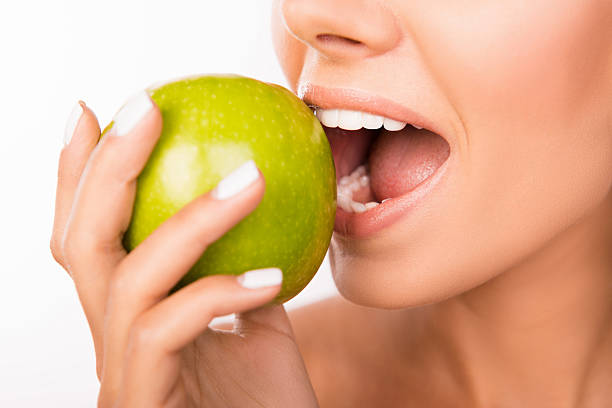
\includegraphics[width=0.5\linewidth]{istockphoto-622282400-612x612.jpg}
    \end{block}
    \vfill
    \begin{columns}[t]
      \begin{column}{.30\linewidth}
        \begin{block}{Introduction}
          \begin{itemize}
          \item some items
          \item some items
          \item some items
          \item some items
          \end{itemize}
        \end{block}
      \end{column}
      \begin{column}{.48\linewidth}
        \begin{block}{Introduction}
          \begin{itemize}
          \item some items and $\alpha=\gamma, \sum_{i}$
          \item some items
          \item some items
          \item some items
          \end{itemize}
          $$\alpha=\gamma, \sum_{i}$$
        \end{block}

        \begin{block}{Introduction}
          \begin{itemize}
          \item some items
          \item some items
          \item some items
          \item some items
          \end{itemize}
        \end{block}

        \begin{block}{Introduction}
          \begin{itemize}
          \item some items and $\alpha=\gamma, \sum_{i}$
          \item some items
          \item some items
          \item some items
          \end{itemize}
          $$\alpha=\gamma, \sum_{i}$$
        \end{block}
      \end{column}
    \end{columns}
  \end{frame}
\end{document}

